%! TEX root=./proposal.tex

\subsection{研究背景和科学意义}

% 第一版
\begin{comment}
% 1. 【描述医疗信息系统发展的现状、设计的初衷、可作为分析平台(副产出)】(统计
%    数据)
随着医疗卫生事业的发展,电子病历系统已成为医院信息系统的核心。电子病历系统在优化
医院工作流程、提高医疗服务质量和搭建区域医疗卫生平台等方面都具有重要的作用。电子
病历在一些发达国家已经有了较深的研究和应用,部分发达国家已经成立了各种政府和民间
的研究机构,开展电子病历的标准化制定工作。电子病历系统的飞速发展,一方面,推动了
医疗机构的信息化建设,使得医院的工作效率和诊疗质量得到了极大的提高。另一方面,经
过多年的发展,电子病历系统已颇具规模,可为医学研究提供新的信息平台,已成为重要的
国家战略资源。近年来,人工智能技术得到了飞速发展,在计算机视觉、自然语言处理、语
音处理等领域都取得了巨大的突破。利用人工智能技术深入挖掘电子病历,发展智能医疗已
成为全球科技趋势,是智能医疗的重要组成部分。 

随着政府、学术界和工业界对智能医疗的重视和投入,近年来相关研究也越来越多。得益于
电子病历系统的先发优势,发达国家在医疗数据质量和医院信息技术方面领先我国,面向医
疗数据的研究开展得较早。IBM是最早布局智能医疗的公司,2013年2月,IBM宣布Watson系
统~\footnote{https://www.ibm.com/watson-health}的第一个商业应用是在肺癌治疗中提
供管理决策,通过快速筛选相似肺癌患者,为医生提供参考的治疗方案。2018年11年,
Google公司宣布成立Google Health部门~\footnote{https://health.google/},并将
DeepMind公司的健康部门及其业务整合其中。目前,Google Health部门已经在眼部疾病、
肺癌、乳腺癌和电子医疗记录分析等领域展开研究并取得一些初步结果。微软亚洲研究院于
2015年11月启动eHuatuo项目
~\footnote{https://www.microsoft.com/en-us/research/project/ehuatuo-teaching-computer-to-read-medical-records/},
致力于病理切片分析、医疗文本分析和知识图谱等研究方向。

% 2. 【国家的政策、医疗数据分析的前景】
%2019年3月,国家卫生健康委发布《国家卫生健康委办公厅关于印发医院智慧服务分级评估
%标准体系(试行)的通知》,提出\textbf{建立0\textasciitilde 5级医疗机构智慧服务
%分级评估体系}。紧接着,

我国卫生部于2010年10月下发了《卫生部关于开展电子病历试点工作的通知》
~\footnote{http://www.gov.cn/gzdt/2010-10/14/content\_1722508.htm},在我国22个省
部分区域和医院开展电子病历试点工作,标志着我国电子病历迈入了一个新的阶段。2017年
7月,国务院《新一代人工智能发展规划》指出\textbf{智能医疗}、\textbf{智能健康和养
老}是未来智能社会的核心组成部分,使``人们能够最大限度享受高质量服务和便捷生活
''。2019年4月,国家卫生健康委和国家中医药管理局联合印发《全国基层医疗卫生机构信
息化建设标准与规范(试行)》,该《规范与标准》针对目前基层医疗卫生机构信息化建设
现状,着眼未来5\textasciitilde 10年基层医疗卫生机构信息化建设、应用和发展要求,
\textbf{鼓励基层医疗卫生机构积极推进云计算、大数据、人工智能等新兴技术应用}。在
国家的宏观部署和政策支持下,大量的研究机构和公司开始投入智能医疗研究,并积极打造
能够落地的医学人工智能应用。作为首批国家人工智能开发平台之一,腾讯觅影
~\footnote{https://miying.qq.com/official/}在癌症早筛、智能导诊和病案管理等方面
都利用人工智能技术取得了突破。为助力今年的新冠疫情,阿里巴巴达摩院开发了CT智能诊
断系统,``截止2020年2月23日,达摩院AI已对3万个临床疑似新冠肺炎病例CT影像进行了诊
断,单个病例影像分析可在20秒内完成,准确率达到
96\%''~\footnote{http://www.sh.chinanews.com/yljk/2020-02-23/71707.shtml}。越来
越多成功的智能医疗系统已陆续在医院开始应用。
\end{comment}

随着医疗卫生事业的发展,电子病历系统已成为医院信息系统的核心组成部分,在优化医院
工作流程、提高医疗服务质量和搭建区域医疗卫生平台等方面都具有重要的作用。上世纪90
年代,国外发达国家已开始建设电子病历系统~\footnote{https://www.nethealth.com/a-history-of-electronic-medical-records-infographic/},
2010年,我国卫生部下发了《卫生部关于开展电子病历试点工作的通知》~\footnote{http://www.gov.cn/gzdt/2010-10/14/content\_1722508.htm},正式布局我国电子
病历系统的建设。经过多年发展,电子病历数据已颇具规模,可为相关研究提供新的数据
平台,成为重要的国家战略资源。

近年来,人工智能飞速发展,在计算机视觉、自然语言处理、语音处理等领域都取得了巨大
的突破。利用人工智能技术分析挖掘电子病历数据有助于改善医疗服务质量,具有重要的商
业价值和社会意义,逐渐得到学术界和工业界的重视,许多研究工作将通用的图像处理和文
本处理模型应用于医学影像和文本,在自动阅片~\citess{wang201901,litjens2017survey,cheplygina2019not}和文本病历实体识别~\citess{leaman2015challenges,wang201902,Lee2019BioBERT}等方面取得了很好的成果。
\textbf{但目前的研究主要集中于医学影像和文本病历,针对电子医疗记录(Electronic
Medical Records, EMRs)的研究相对较少,缺少针对电子医疗记录分析的解决方案}。电子
医疗记录是指有固定格式的、由医生录入的、从患者入院到出院的全部记录,包括检查、诊
断、手术、用药等信息,包括患者一次或者多次就医的全过程信息,\textbf{对电子医疗
记录进行深入分析可以辅助临床决策,有助于优化患者管理和提升医疗服务质量,是未来智能医疗的重要组成部分}~\citess{rajkomar2018scalable,kwak2019deephealth,rajkomar2019machine}。

\cref{fig:ch1:emr}展示了患者就医产生电子医疗记录和基于这些数据进行分析和解释的示
意图。患者在医院的每个记录可以用三元组(\textit{recordID, value, time})来表示,其
中\textit{recordID}是指医疗概念,\textit{value}表示该医疗概念对应的值,
\textit{time}表示记录的时间,以血糖为例,患者血糖被记录时会产生一条记录
(\textit{血糖,7.1mmol/L, 2020-02-29 15:20:32})。\textit{recordID}通常采用医院规
定的标准编码,在不同地区和医院之间有一定的通用性,也是针对电子医疗记录进行分析的
基本特征。患者每次就医产生多条电子医疗记录,即有多个\textit{recordID}被记录下
来,同时,患者可能多次访问医院,因此,如图所示,电子医疗记录可用二维矩阵表示,横
轴表示时间,记录患者去就医的时间,纵轴表示不同的医疗记录编码,包括诊断、检查、手
术和用药等,图中所示的患者患有第二型糖尿病(E11.2),同时伴随有慢性肾脏病第三期
(N18.3)和高血压(R03.0),某次就诊时还患有感冒(J00),就诊时医生会安排检查血压
(BP)、血糖(BG)等指标,确诊后会开药,如图中所示的阿卡波糖(acarbose),阿洛列
汀(alogliptin)等。\textbf{可见,电子医疗记录全面记录了患者就医数据,对其进行深
入分析可以辅助疾病阶段预测、患者风险评估、重入院时间和治疗方案决策等临床工作,不
仅能帮助患者得到及时周到的治疗,还能减轻医务工作者的负担,具有重要的社会意义和商
业价值}。

\begin{figure}%[htbp]
    \begin{small}
        \begin{center}
            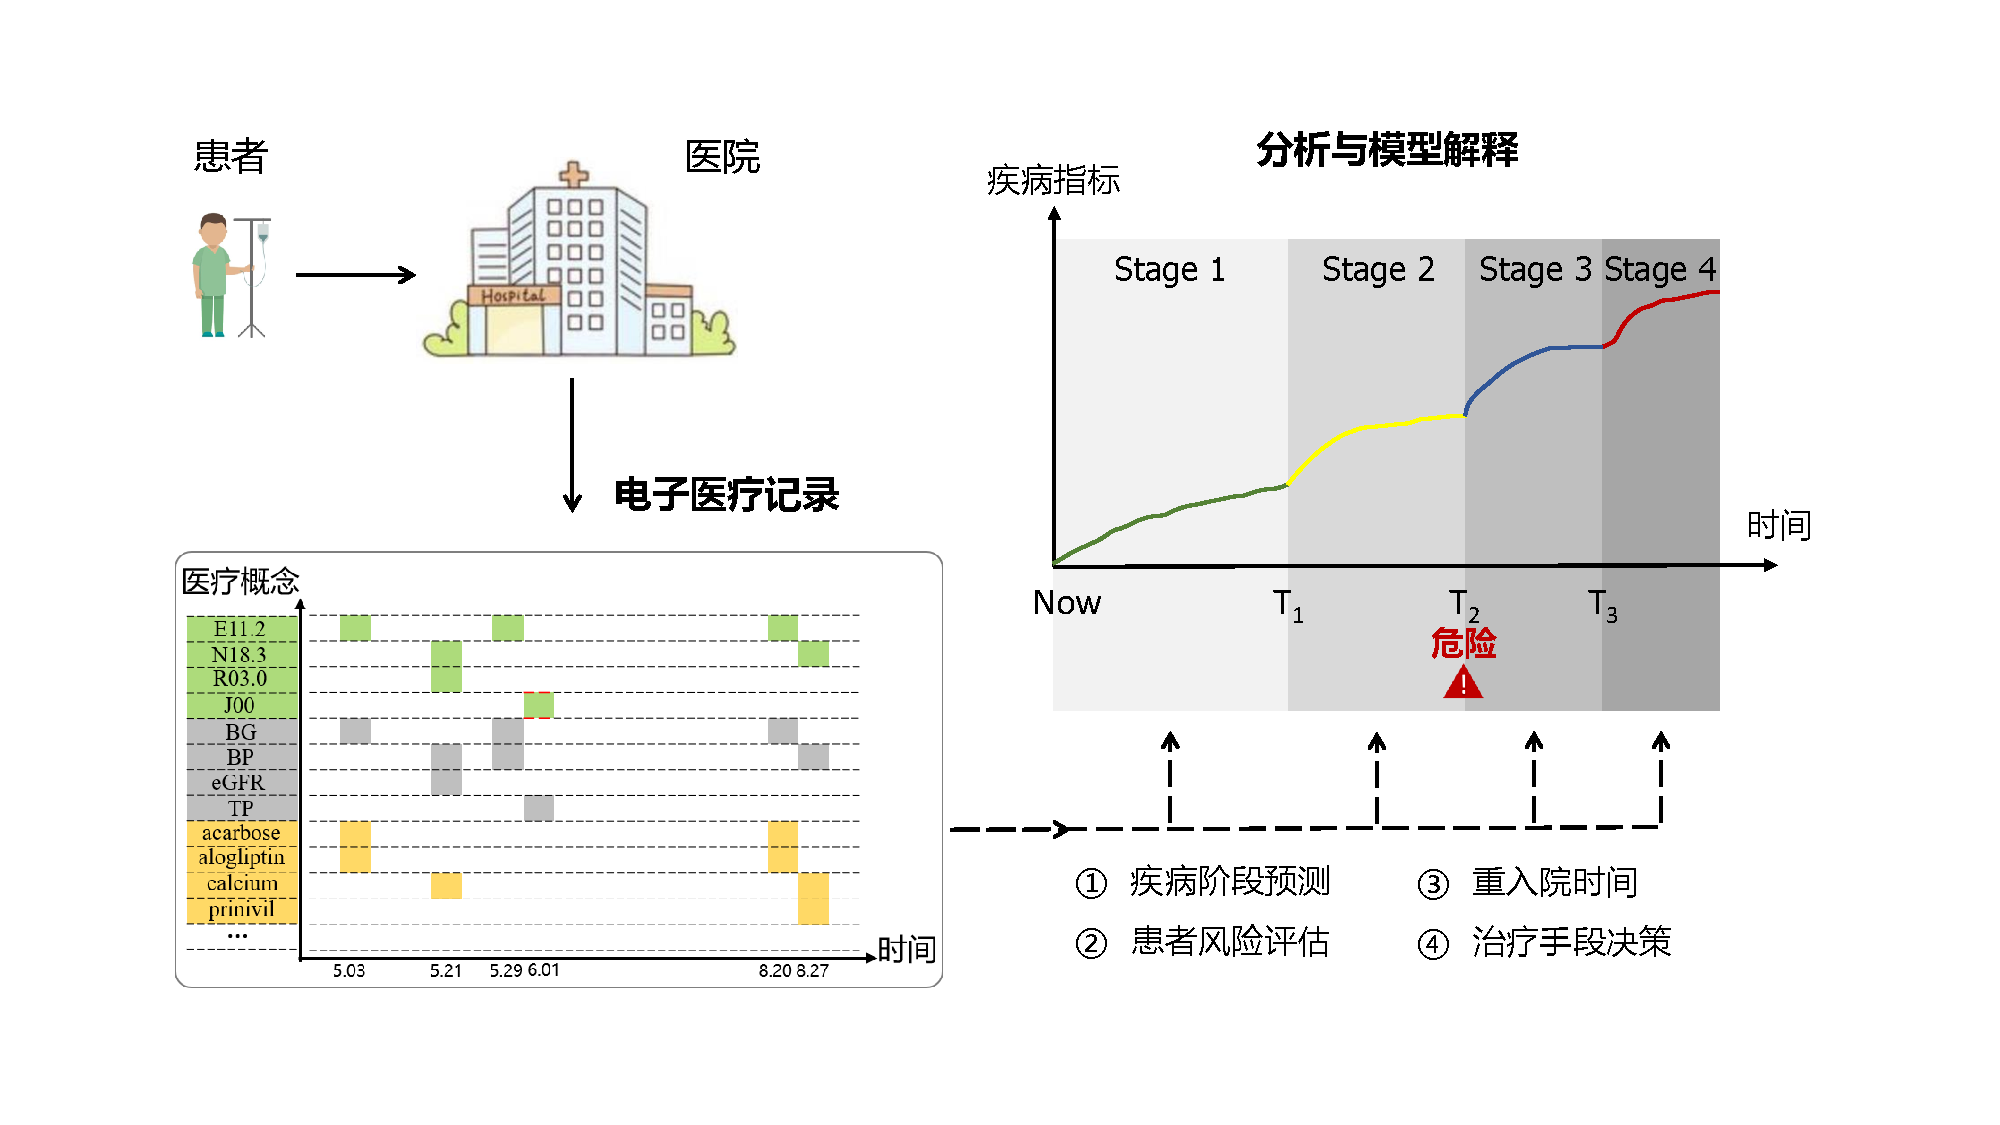
\includegraphics[width=0.9\textwidth]{ch1_emr_analysis.pdf}
        \end{center}
        \caption{电子医疗记录及其分析}
        \label{fig:ch1:emr}
    \end{small}
\end{figure}

结合电子医疗记录的特点和医疗领域的应用需求,可以知道,电子医疗记录分析具有以下挑
战:
\begin{itemize}

    \item[(1)] \textbf{高维性}。电子医疗记录所包含的医疗概念非常多,导致每个患者
    的特征维度非常高,例如:由世界卫生组织整理发布的ICD-10~\footnote{《国际疾病
    与相关健康问题统计分类第十版》(the 10th revision of the International
    Statistical Classification of Diseases and Related Health Problems),
    https://icd.who.int/browse10/2016/en}是常用的疾病诊断编码标准,而ICD-10共包
    含15.5万种编码,即疾病的种类(特征数)已达10万级规模。另一方面,相比总数15.5
    万种疾病,患者实际就诊时的疾病诊断编码只占很小的一部分,这使得如图
    ~\ref{fig:ch1:emr}所示的电子医疗记录是非常稀疏的。此外,电子医疗记录包含的检
    查(LONIC~\footnote{https://loinc.org/})、药物
    (NDC~\footnote{https://www.fda.gov/drugs/drug-approvals-and-databases/national-drug-code-directory})
    等编码同样具有高维性。

    \item[(2)] \textbf{不规则性}。电子医疗记录因为种种原因会有大量的缺失值,如尽
    管医生通常会建议患者去医院的时间,但患者未必遵照医嘱,反而只会在自己不舒服时
    才会去医院就医。另一方面,不同医疗概念的记录频率差别较大,如血糖值需要一天内
    测量多次,但肌酐通常一天内只测量一次。图~\ref{fig:ch1:emr}的示例也反映了电子
    医疗记录在时间维度上具有不规则性,这为直接分析电子医疗记录带来了新的挑战。

    \item[(3)] \textbf{易扰性}。电子医疗记录的特征之间相互作用关系复杂,基于电子
    医疗记录构建的机器学习模型容易被混淆特征(confounder)干扰,例如:早期很多数
    据分析表明口服避孕药和心肌梗塞具有强关联性,但是后来研究发现,这部分节育人群
    种吸烟的比例较高,容易发现,吸烟这个特征混淆了口服避孕药和心肌梗塞的关系。这
    种特征之间的易扰性对构建可解释、可泛化的分析模型带来了巨大挑战,严重影响了模型的临床应用。
\end{itemize}

本项目直接面向国家医疗卫生事业和人工智能的发展战略,结合临床分析任务,研究电子医
疗记录预测性分析的关键技术,从数据获取、数据预处理和数据分析三个方面,基于深度学
习构建面向电子医疗记录的数据分析方案,解决电子医疗记录高维性、不规则性和易扰性所
带来的挑战,提升分析的准确性和可解释性,为基于电子医疗记录的智能医疗服务提供核心
技术支撑。本项目的研究意义主要体现在以下四个方面:

\begin{itemize}
    \item[(1)] \textbf{本项目拟实现基于表现型(phenotype)的自动队列识别方法}。
    队列识别即给定筛选条件,从电子医疗记录中选出一组患者,其中部分患者有某种疾病
    (实验组),而另外一部分没有(对照组),准确的队列识别是电子医疗记录分析的基
    础。但因为电子医疗记录的高维性,加之并发症、异病同治和同病异治等原因,队列识
    别的准确性不高。而且,传统的队列识别需要医生花费大量精力比对患者的记录和统计
    图表才能得到,因此难以获得大规模电子医疗记录的队列标签。表现型是指可以代表患
    者或者疾病特点的一组人体生化或者物理特征,不同疾病通常有其特有的表现型。本项
    目拟针对电子医疗记录,构建基于表现型字典的患者表示模型,同时采用弱监督学习方
    法在模型中引入大规模未标注样本,提高表现型字典和患者的表示学习效果,进而实现
    准确的队列识别。

    \item[(2)] \textbf{本项目拟融合电子医疗记录缺失规律和数值特征,实现电子医疗
    记录缺失值插补的通用方法}。电子医疗记录插补是指将有缺失值的电子医疗记录补全
    为完整的数据。经过插补处理后的电子医疗记录可使用现有循环神经网络(Recurrent
    Neural Network, RNN)及其变种进行建模,能有效缓解数据不规则性带来的影响,提
    升模型效果。如果图~\ref{fig:ch1:emr}所示的电子医疗记录是一个稠密矩阵,数据分
    析师(甚至医生)可以较容易地调用RNN对该数据集建模,实现患者病情的预测。现有
    针对电子医疗记录的插补研究较少,且它们忽略了电子医疗记录中固有的医学偏差
    (medical bias),导致插补后的数据不够准确。本项目以特征缺失规律反映医学偏
    差,通过对偶RNN模型融合缺失规律和观察到的数值特征,实现更准确、泛化能力更强
    的电子医疗记录插补模型。

    \item[(3)] \textbf{本项目拟结合特征重要性和时间关联性解释模型行为和预测结
    果,构建基于深度学习的可解释预测模型,助力模型落地临床应用}。有别于静态数据
    分析,电子医疗记录的可解释性需要考虑数据中存在的时间信息,不同医疗概念的时间
    作用域不同,如对于糖尿病患者来说,其较高的血糖值持续出现的时间较长,而对于非
    糖尿病患者,血糖值虽然也可能会偏高,但持续时间较短,所以如果在多个时间点出现
    高血糖值,该患者更有可能患有糖尿病。由于时间维度的复杂性,现有针对电子医疗记
    录分析的可解释模型未充分考虑特征的重要性和时间关联性,无法得到模型全面的解
    释,本项目拟通过结合这两者,不仅可以解释给定病例的预测结果,还能总结与预测目
    标相关的临床路径(clincial pathway),反哺医学研究。

    \item[(4)] \textbf{本项目拟在慢性肾病进展预测和感染性休克预警两个临床任务上
    验证上述方案的可行性}。(a) 随着糖尿病患者的增加,与糖尿病有关的慢性肾病
    (DKD)患者近年来也显著增加,据研究者估计,截止2016年,我国至少有2430万DKD患
    者~\citess{zhang2016trends}。本项目拟与北京大学医疗健康大数据国家研究院合
    作,在真实慢性肾病电子医疗记录上预测患者的病情发展情况,辅助医生对部分患者及
    早进行临床干预。(b) 感染性休克是急诊科常见的急危重症,流行病学研究显示,急诊
    患者中,7.3\%在入住4h内发生严重感染,12\%的严重感染患者在入住48h内发展为感染
    性休克,及时预测或发现病人的状态对降低ICU感染性休克的病发率和死亡率具有重要
    意义。本项目拟在麻省理工学院公开的ICU数据集
    MIMIC-III~\citess{johnson2016mimic}上,通过预测感染性休克验证本项目的研究成
    果。
\end{itemize}

\subsection{国内外研究现状及发展动态分析}\label{relatedwork}

根据与本项目的相关性,本节从电子医疗记录的表示学习、表现型分析、数据插补、以及模
型的可解释性四个方面介绍和分析国内外研究现状。

%(1) \textbf{电子医疗记录表示学习}
\subsubsection{电子医疗记录表示学习}

电子医疗记录的表示学习借鉴于自然语言处理领域的词嵌入(word embedding),尤其是
word2vec~\citess{mikolov2013efficient,mikolov2013distributed}模型。表示学习的基
本思想是:出现在相似上下文的特征具有相似的语义信息,即相似的向量表示。好的医疗特
征表示能合理地反映医疗特征之间的语义关系,有助于电子医疗记录的分析。

基于电子医疗记录的表示学习研究工作如\cref{tab:representation}所示。Tran等人~\citess{tran2015learning}利用非负玻尔兹曼机(Nonnegative Restricted Boltzman
Machine)学习医学特征的向量表示,是最早使用深度学习的研究方法;Miotto等人~\citess{miotto2016deep}和Choi等人~\citess{choi2016medical}也较早的利用其他深度
学习模型学习学习医疗特征的表示;\textbf{本项目申请人蔡祥睿~\citess{cai2018medical}首先提出不同医疗特征的时间作用域有差别,其上下文界定不能
设置为固定超参数,并引入注意力机制,学习医疗特征不同的上下文时间范围};Peng等人~\citess{peng2019temporal}在此基础上设计更复杂的注意力模型,进一步提高特征表示学
习的效果。这些工作所使用的数据只有电子医疗记录数据集;Bai等人~\citess{bai2019medical}提出对齐多医疗机构的特征并学习其表示。Choi等人~\citess{choi2017gram,choi2018mime}率先在医疗特征表示学习模型中引入领域知识;Ma
等人~\citess{ma2018kame}也提出了相似的思路,并将所学特征表示用于疾病诊断的预测;
Song等人~\citess{song2019medical}面向多个机构的电子医疗记录表示学习,通过引入了
医学领域的知识库进行语义对齐。部分研究工作通过结合电子医疗记录、病历和文献等异构
数据进行模型训练,期望得到更好的特征表示~\citess{choi2016learning,bai2017joint,ma2018drug}. 此外,Choi等人还提出了针对医
疗特征和患者就诊两个层次的表示学习模型~\citess{choi2016multi},以及利用图神经网
络学习医疗特征之间的关联关系~\citess{choi2020learning},这些工作在医疗特征表示学
习中引入了数据的结构知识。

\begin{table}
    \renewcommand\arraystretch{1.5}
    \begin{small}
        \caption{EMR表示学习相关研究工作}
        \label{tab:representation}
        \begin{center}
            \begin{tabular}[c]{cll}
                \toprule
                \multicolumn{1}{c}{\textbf{序号}} & 
                \multicolumn{1}{c}{\textbf{主要思想}} &
                \multicolumn{1}{c}{\textbf{文献号}}\\
                \midrule
                1 & 仅基于EMR数据集训练医疗特征表示 & \cite{tran2015learning}
                \cite{miotto2016deep} \cite{choi2016medical}
                 \cite{cai2018medical} \cite{peng2019temporal}
                 \cite{bai2019medical}\\
                2 & 结合EMR数据集和医疗领域知识库 & \cite{choi2017gram}
                \cite{choi2018mime} \cite{ma2018kame} \cite{song2019medical}\\
                3 & 基于异构医疗数据学习医疗特征表示 & \cite{choi2016learning}
                \cite{bai2017joint} \cite{ma2018drug}\\
                4 & 学习层次化的EMR数据表示 & \cite{choi2016multi}
                \cite{choi2020learning}\\
                \bottomrule
            \end{tabular}
        \end{center}
    \end{small}
\end{table}

{\kaishu{电子医疗记录中特征表示与表现型直接相关,是队列识别的重要研究问题之一,
特征表示是表现型表示和队列识别的基础。现有工作主要聚焦于针对医疗特征的向量表示学
习研究,缺少对高层次语义表示的研究,如表现型表示。本课题拟引入表现型向量字典,将
患者表示为多个高层次表现型的组合,从而提升队列识别的准确率。}}

\subsubsection{电子医疗记录表现型分析}

表现型是一组患者或者疾病的属性,根据表现型不同可以将患者划分成更有意义的分组,与
本项目研究内容队列识别直接相关。面向电子医疗记录的表现型分析的主要方法如
\cref{tab:phenotype}所示。

针对电子医疗记录进行表现型分析的人物最早由现在UIUC的Jimeng Sun教授团队引入计算机
领域,他们将电子医疗记录看作张量,利用张量分解进行降维分析~\citess{ho2014extracting},随后,该团队还先后将基于张量分解的模型扩展到联邦学习~\citess{kim2017federated}和无监督学习~\citess{perros2018sustain}的场景中,由于
电子医疗记录的高维性,张量分解的效率较低,Heano等人~\citess{heano2018parallel}和
He等人~\citess{he2019distributed}研究如何利用并行和分布式技术进行加速。基于张量
分解的模型缺乏对记录时间的考虑,部分研究工作将电子医疗记录建模成图,图中的点为医
疗特征,特征记录如果相邻,则给图增加一条对应的边,边的权重与记录时间间隔相关,最
后利用图算法分析患者的表现型,如图分解~\citess{liu2015temporal}、频繁子图挖掘~\citess{wang2015graph,xu2017predicting}等方法。深度学习模型擅长表示学习,非常适
合表现型分析,同时,挖掘表现型也能提高深度学习模型的可解释性~\citess{kale2015causal}。Che等人~\citess{che2015deep}较早的将医疗编码的层次结构
引入基于深度学习的表现型分析模型;Beaulieu-Jones等人~\citess{beaulieu2016semi}提
出基于去噪自编码器的半监督模型,不需要大量标注样本,是本项目的重要参考;Baytas等
人~\citess{baytas2017patient}利用表现型对患者进行细粒度的划分;Fu等人~\citess{fu2019ddl}首次提出面向表现型的深度字典学习,为本项目引入表现型字典提供
了理论依据;Seymour等人~\citess{seymour2019derivation}利用深度学习研究感染性休克
的表现型,是本项目研究感染性休克预测的重要参考。

\begin{table}
    \renewcommand\arraystretch{1.5}
    \begin{small}
        \caption{针对EMR的表现型分析方法}
        \label{tab:phenotype}
        \begin{center}
            \begin{tabular}[c]{cll}
                \toprule
                \multicolumn{1}{c}{\textbf{序号}} & 
                \multicolumn{1}{c}{\textbf{主要思想}} &
                \multicolumn{1}{c}{\textbf{文献号}}\\
                \midrule
                1 & 以张量表示EMR数据集,进行张量分解 &
                \cite{ho2014extracting} \cite{kim2017federated}
                \cite{perros2018sustain} \cite{heano2018parallel} \cite{he2019distributed}
                \cite{perros2019temporal} \\
                2 & 将EMR建模成图,利用图算法分析表现型 & \cite{liu2015temporal}
                \cite{wang2015graph} \cite{xu2017predicting} \\
                3 & 基于深度学习模型,多为监督学习 & \cite{kale2015causal}
                \cite{che2015deep}
                \cite{beaulieu2016semi} \cite{cheng2016risk} 
                \cite{baytas2017patient} \cite{fu2019ddl} \cite{seymour2019derivation} \\
               \bottomrule
            \end{tabular}
        \end{center}
    \end{small}
\end{table}

{\kaishu {现有基于深度学习的表现型分析模型绝大多数都是有监督模型,需要大量的标注
样本,难以在真实医疗场景中应用。值得注意的是,部分研究工作直接基于医疗特征表示进
行队列识别,如~\cite{glicksberg2018automated,bai2018ehr},由于电子医疗记录的高维
性,这类方法容易得到相似度较高的患者表示,不利于队列识别。}}

\subsubsection{电子医疗记录插补}

因为患者就医时间没有规律,电子医疗记录呈现时间不规则性,直接利用现有模型分析电子
医疗记录难以取得较好的结果,因此,数据插补对电子医疗记录的分析具有重要意义。关于
电子医疗记录插补的相关工作总结如\cref{tab:imputation}所示。

针对数据缺失值的插补很早就被关注,最传统的方式是利用均值、中位数进行插补,但缺乏
对数据分布的考虑,效果较差。基于传统机器学习模型进行插补近年来也一直有研究者在关
注,Beaulieu-Jones等人~\citess{beaulieu2018characterizing}在电子医疗记录上对比了
12中传统机器学习模型方法,发现MICE~\citess{sterne2009multiple}很多情况下能取得较
好的结果。值得注意的是,Zheng等人~\citess{zheng2017resolving}较早的提出了要考虑
电子医疗记录中的医学偏差,并利用隐马尔可夫模型加入对偏差的考虑,但该工作只推断患
者的状态,不能得到缺失值的插补。随着深度学习的发展,越来越多的研究工作开始利用深
度学习模型处理电子医疗记录中的缺失值,Che等人~\citess{che2018recurrent}较早地利
用RNN模型进行电子医疗记录插补,为考虑时间不规则性的影响,他们设计了时间衰减因
子,Cao等人~\citess{cao2018brits}和Suo等人~\citess{suo2019recurrent}构建更复杂的
RNN模型,进一步提升\cite{che2018recurrent}的效果。除了RNN模型,少量研究工作也以
AutoEncoder为主干模型,实现电子医疗记录插补~\citess{beaulieu2017missing,costa2018missing}。\textbf{最近,本项目申请人首先提
出将插补问题看成数据生成问题,并构建基于生成对抗网络(Generative Adversarial
Network,GAN)的数据插补模型~\citess{luo2018multivariate,luo20192},在该领域取得
了国际领先结果}。此外,Yoon等人~\citess{yoon2018gain}同样利用GAN进行数据插补,
Mattei等人~\citess{mattei2019miwae}首次在本问题上采用深度隐变量模型(Deep Latent
Variable Model),但它们的数据假设局限于完全随机缺失(Missing Completely At
Random)和非时序数据,无法应用于电子医疗记录。

\begin{table}
    \renewcommand\arraystretch{1.5}
    \begin{small}
        \caption{EMR插补相关研究工作}
        \label{tab:imputation}
        \begin{center}
            \begin{tabular}[c]{cll}
                \toprule
                \multicolumn{1}{c}{\textbf{序号}} & 
                \multicolumn{1}{c}{\textbf{主要思想}} &
                \multicolumn{1}{c}{\textbf{文献号}}\\
                \midrule
                1 & 传统机器学习模型 & \cite{zheng2017resolving}
                \cite{beaulieu2018characterizing} \cite{yang2018time} \cite{xu2019estimating} \cite{sterne2009multiple}
                \\
                2 & 基于RNN的缺失值预测模型 & 
                \cite{che2018recurrent} \cite{suo2019recurrent}
                ~\cite{cao2018brits} \\
                3 & 基于AutoEncoder模型重构缺失值 & \cite{beaulieu2017missing}
                \cite{costa2018missing} \\
                4 & 基于生成模型进行缺失值生成 & \cite{luo2018multivariate}
                \cite{luo20192} \cite{yoon2018gain} \cite{mattei2019miwae} \\
               \bottomrule
            \end{tabular}
        \end{center}
    \end{small}
\end{table}

电子医疗记录中的偏差是医学领域中的常见问题,已经被许多医学研究证实:Pivovarovd等
人~\citess{pivovarov2014identifying}利用特征出现的频率识别临床检测数据中的偏差,
Phelen等人~\citess{phelan2017illustrating}举例说明了电子医疗记录中医学偏差产生的
原因,Agniel等人~\citess{agniel2018biases}设计回顾性分析实验,证明了医学偏差在电
子医疗记录中普遍存在,Vassy等人~\citess{vassy2018yield}利用可视化分析发现偏差。
这些研究结果指出,医学偏差可以作为一种特征,有助于理解数据。

{\kaishu{本项目拟将医学偏差作为患者分布的特征,通过将其引入电子医疗记录插补模
型,实现隐式地进行细粒度患者划分,提高数据插补的准确性。目前已有研究可以佐证引入
医学偏差能提高模型效果,但尚未有相关研究在基于深度学习的插补模型中引入医学偏差,
本项目的研究正好补充该方向上的空白。}}

\subsubsection{模型可解释性}

拥有良好的可解释性是机器学习模型实际应用的重要保证,这在医疗数据分析领域尤其重
要。虽然目前越来越多的研究工作开始利用深度学习对电子医疗记录建模,但可解释性是深
度学习的基础性难题,尚无非常完备的解决的方案。\cref{tab:interpretability}总结了
电子医疗记录分析模型可解释性的研究。现有关于电子医疗记录分析的可解释性研究主要分
为两类:1)将模型看作黑盒(black-box),待模型训练完以后再对分析结果进行解释
(Post-hoc);2)改进模型,使模型本身具有可解释性(Ante-hoc)。除了这两类模型方
面的研究以外,也有一些工作研究可视化交互界面,建立人机互动的平台。

\begin{table}
    \renewcommand\arraystretch{1.5}
    \begin{small}
        \caption{EMR模型可解释性相关研究工作}
        \label{tab:interpretability}
        \begin{center}
            \begin{tabular}[c]{cll}
                \toprule
                \multicolumn{1}{c}{\textbf{序号}} & 
                \multicolumn{1}{c}{\textbf{主要思想}} &
                \multicolumn{1}{c}{\textbf{文献号}}\\
                \midrule
                1 & 将模型看作黑盒,对预测结果进行解释(Post-hoc) & \cite{panigutti2019explaining}
                \cite{panigutti2020doctor} \\
                2 & 修改模型结构,在预测同时提供可解释性(Ante-hoc) &
                \cite{choi2016retain} \cite{ma2017dipole} \cite{bai2018interpretable}
                \cite{gao2019camp} \cite{ma2019adacare} \\
                3 & 利用可视化界面,便于理解 & \cite{kwon2018retainvis} \cite{jin2020carepre}
                \cite{guo2020comparative} \\
                \bottomrule
            \end{tabular}
        \end{center}
    \end{small}
\end{table}

LIME~\citess{ribeiro2016should}最早提出将模型看作黑盒,并逐样本解释预测结果的方
法;Panigutti等人~\citess{panigutti2019explaining}首先利用这种方法解释电子医疗记
录分析模型,但该工作解释的模型缺少时间属性;随后,他们由针对考虑时间的模型应用相
同的思想,提出了Doctor XAI~\citess{panigutti2020doctor}。这类方法的核心思想是利
用给定样本周边的样本训练一个简单模型,以此对原模型预测的可靠性做出解释,方法无法
给出原模型决策的原因。我们知道,对抗样本仅对原样本做了一点微小的改变,却能改变模
型预测结果~\citess{su2019one},因此Post-hoc的方法难以在医疗领域广泛应用。

Ante-hoc方法主要是通过注意力机制对模型进行改造,使其具有可解释性。
Choi~\citess{choi2016retain}于2016年提出RETAIN模型,将RNN隐含层的部分计算转移给
注意力机制,虽然一定程度上提高了模型可解释性,但其预测准确率较低;Bai等人~\citess{bai2018interpretable}和Ma等人~\citess{ma2019adacare}分别提出了针对
RETAIN模型的改进。Dipole模型~\citess{ma2017dipole}只能提供关于预测目标比较的重要
就医记录(一次就医的所有记录),无法进一步细粒度分析。这些模型仅考虑了动态特征,
忽略了静态特征的影响。Gao等人~\citess{gao2019camp}虽然同时考虑了静态特征和动态特
征,但两组特征的重要性是分别计算的,没有得到全局下的特征权重,而且该模型无法总结
出模型的行为准则,每个病历需要单独判别。

在可视化医疗分析平台方面,Kwon等人~\citess{kwon2018retainvis}为RETAIN做了可视化
界面;Jin等人~\citess{jin2020carepre}提出了交互式的智能医疗决策辅助平台CarePre;
而Guo等人~\citess{guo2020comparative}聚焦于可视化电子医疗记录,为基于不同队列的
对比研究提供辅助。这些可视化分析方法和平台,是本项目系统研发的重要参考。



{\kaishu{现有可解释性研究无法对模型的预测行为进行全局分析,本项目拟提出可溯源的
电子医疗记录分析模型,通过同时比较静态特征和动态特征对预测结果的贡献,可从整体上
分析特征的变化对模型的影响。此外,本项目拟研发可视化界面呈现模型可解释分析结
果。}}

% 因为写 demo,我把参考文献放这里了,真写本子的时候,还是要放在国内外概况那边
\begin{spacing}{1.3} % 行距
	\zihao{5} \songti   
	\bibliographystyle{gbt7714-nsfc}
	\bibliography{ref}  
	\vspace{11bp}
\end{spacing}